\documentclass[12pt,a4paper]{article}
\usepackage{ctex}
\usepackage{graphicx}
\usepackage{geometry}
\usepackage{array}
\usepackage{setspace}
\usepackage{xeCJK}
\usepackage{indentfirst}
\usepackage{amsmath}
\usepackage{amsthm}
\usepackage{float}
\usepackage{subfigure}
\usepackage{booktabs}
\usepackage{multirow}
\usepackage{caption}

% 页边距
\geometry{left=2.5cm,right=2.5cm,top=2.5cm,bottom=2.5cm}

% 默认宋体小四
\setCJKmainfont[BoldFont=SimHei]{SimSun}
\zihao{-4}
\linespread{1.5} % 小四字通常 1.25 倍行距更接近 Word 默认

\begin{document}

% 实验名称（小二黑体、居中）
\begin{center}
  {\zihao{2}\heiti 全息照相与激光全息}
\end{center}

% 年级 专业 姓名 座位号（宋体小四、居中、段前后 0.5 行）
\vspace{0.5\baselineskip}
\begin{center}
  （\textbf{年级}\ \underline{2024 级}\quad \textbf{专业}\ \underline{x} \quad \textbf{姓名}\ \underline{Pinco Li} \quad \textbf{座位号} \ \underline{5}）
\end{center}
\vspace{0.5\baselineskip}


% 实验目的部分标题
\textbf{一、实验目的}

{\setstretch{1.0}
\begin{enumerate}
    \item 了解全息照相的基本原理和特点
    \item 学习静态全息照相的拍摄方法和有关技术
    \item 掌握全息照相再现物像的性质和观察方法
    \item 理解激光在全息技术中的重要作用
\end{enumerate}
}

\textbf{二、实验仪器}

{\setstretch{1.0}
\begin{itemize}
    \item 光学实验台
    \item 氦氖激光器
    \item 分束镜
    \item 扩束镜
    \item 反射镜
    \item 载物台
    \item 各种镜头支架
    \item 被摄物体
    \item 全息干板
    \item 暗室冲洗胶片器材
\end{itemize}
}

\begin{figure}[H]
    \centering
    \includegraphics[width=0.6\textwidth]{assets/IMG_20250909_095229.jpg}
    \caption{全息照相实验仪器}
\end{figure}

\textbf{三、实验原理}

\textbf{1. 全息照相的发展历史}

早在1948年匈牙利裔英国物理学家丹尼斯·伽博就已经做出了第一张全息照片。他当时用高压汞灯作为光源，但在实验中一直受到偶偶全息像的困扰，有效的工作很少。因此20世纪50年代中期，全息术的研究工作一直处于停顿状态。1960年激光器的出现给全息术带来了新的生命。1962-1963年，利斯和乌帕特尼克斯共同发表了第一张激光全息图，立刻引起了轰动。1964年他们又用光照明漫反射物体制作全息图，成功地得到了三维物体的立体再现像。他们提出的斜参考波法应用子激光全息，取得了全息技术的重大突破。1971年伽博因全息术的发明而获得了诺贝尔奖。

全息技术发展到现在可分为三代：第一代全息术为同轴全息，用水银灯记录，光源相干性差，原始像与共轭像分不开；第二代全息技术为离轴全息，用激光记录，激光再现，原始像与共轭像分离，可以再现具有三维特性的立体像；第三代全息是用激光记录，白光再现的全息术，主要有反射全息、像面全息、彩虹全息以及合成全息等。本实验我们学习第二代全息术并制作全息照片。

\textbf{2. 全息照相基本原理}

全息照相是一种用光学方法在视觉上再现清晰立体像的典型技术，全息照相分为两步：波前记录和波前再现。波前记录是指将物体射出（直接或间接）的光波与另外一束相干光波（参考光波）相干涉，用照相的方法将干涉条纹记录下来，称全息图。当用原光路时的参考光或其他合适的激光照射全息图时，光通过全息图发生衍射，其衍射光波与原物体的光波相似，于是构成物体的再现，这就是波前再现。

\begin{figure}[H]
    \centering
    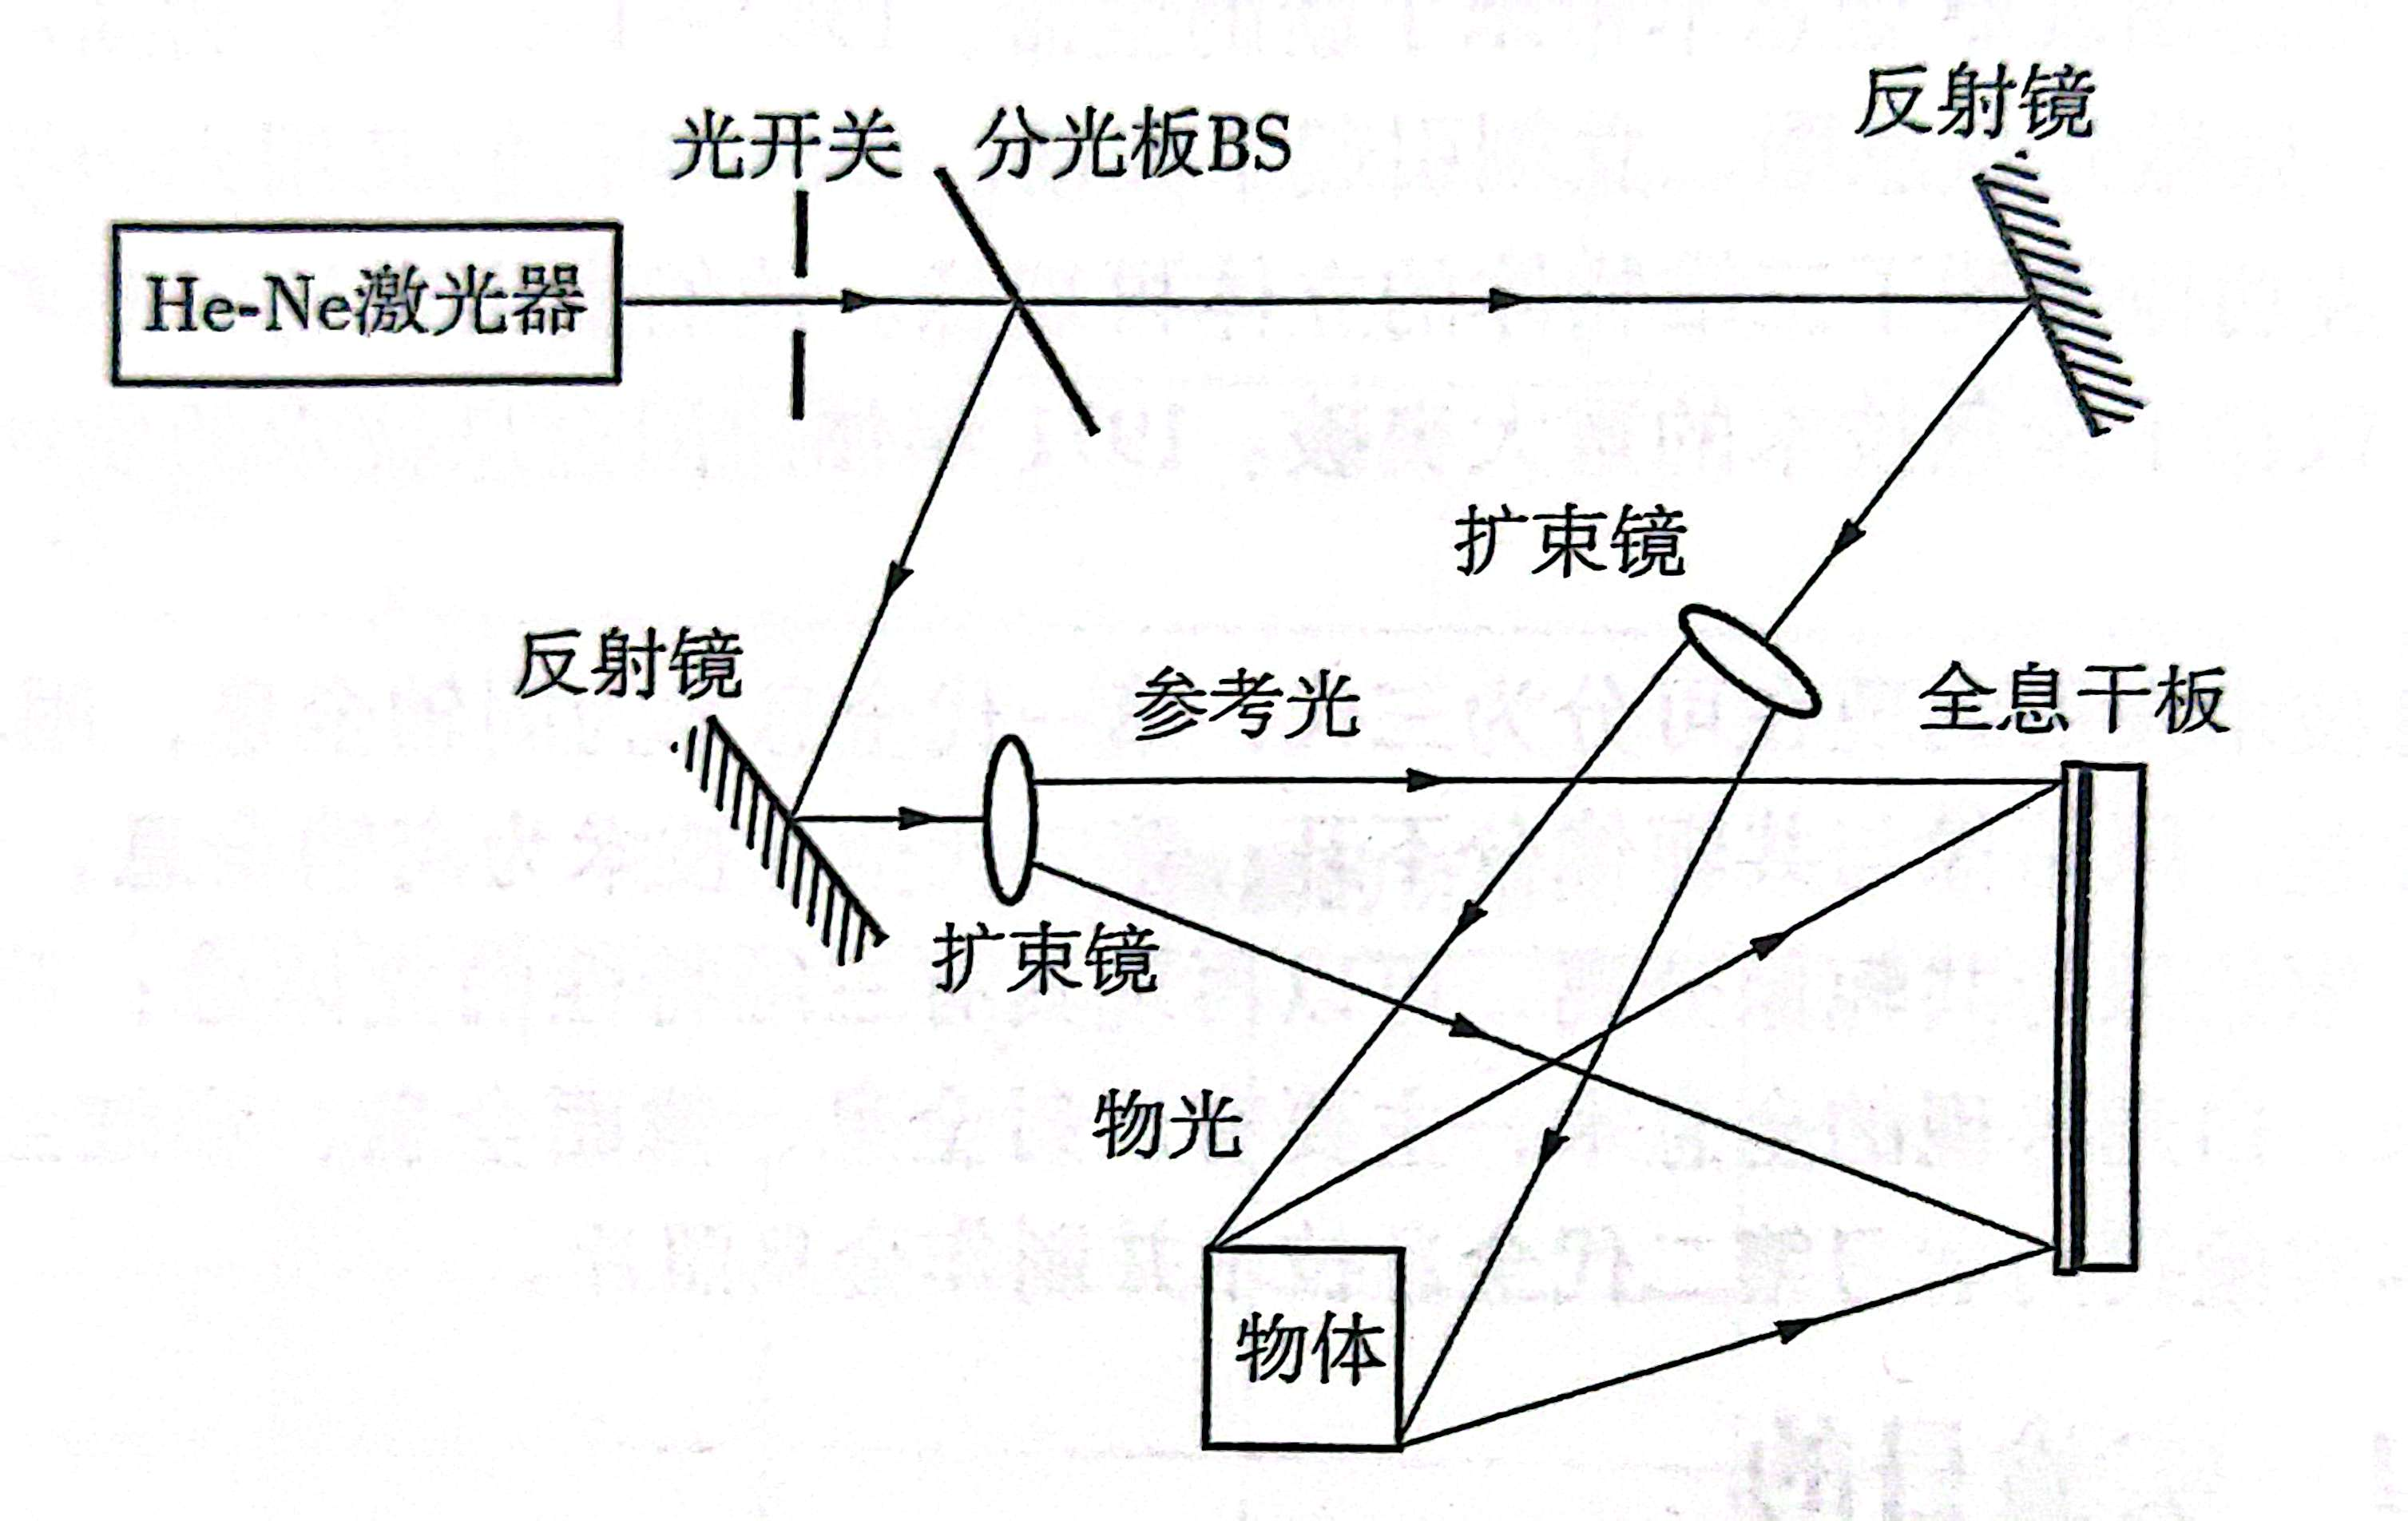
\includegraphics[width=0.6\textwidth]{assets/Figure_1.jpg}
    \caption{全息照相成像光路}
    \label{fig:holography_principle}
\end{figure}

\textbf{3. 全息记录原理}

待记录的物光波载有物体特征的信息，构成一种复杂的光路，其复振幅可表示为：

\begin{align}
    O(x,y) = O_{0}(x,y) e^{j\varphi_{0}(x,y)} = O_{0} e^{j\varphi_{0}}
\end{align}

式中，$O(x,y)$是记录介质平面上的坐标，$O_0(x,y)$和$\varphi_0(x,y)$分别是参考光在$(x,y)$处的振幅和相位。

与此类似，参考光波可表示为

\begin{align}
    R(x,y)=R_0(x,y)e^{i\phi_r(x,y)} =R_0e^{i\phi_r}
\end{align}

记录时物光和参考光在记录介质平面上相干叠加后的光强分布为

\begin{align}
    I(x,y)=|O+R|^2 = (O+R)(O^*+R^*)
\end{align}

\begin{align}
    =O_0^2+R_0^2+O_0R_0 e^{i(\phi_0-\phi_r)} +O_0R_0e^{i(\phi_r-\phi_0)}
\end{align}

从式中可以看出，物光振幅$O_0$与相位$\phi_0$已经以光强的形式被记录下来，第一项是背景光强度；后两项的大小随物性变化的，是与时间无关的干涉相，包含了物光的相位信息，因此物光波的相位信息就这样转化成了强度信息。

\textbf{4. 全息再现原理}

对于薄型全息图，显影过程中要产生一个表征全息图振幅透过率的函数：

\begin{align}
    T(x,y)=FI(x,y)
\end{align}

记录介质不同，函数$F[I(x,y)]$可以是实函数、虚函数或复函数，同时，它可以是线性的也可以是非线性的，但无论何种情况下都可以进行线性近似。对于振幅型全息图，便可得到一个透射函数：

\begin{align}
    T(x,y)=T_0+\beta I(x,y)
\end{align}

式中，$T_0$是代表背景的一个常数，$\beta$是与材料性质和曝光时间有关的比例系数。

再现过程通常是采用与参考光完全相同的读出光去照明全息图，读出光波可用$R(x,y)$表示，则在全息图后表面的光场分布可表示为

\begin{align}
    W(x,y)=R(x,y)T(x,y)=R_0^2R_0e^{i\phi_r}+\beta T_0 R_0e^{i\phi_r}+\beta O_0R_0^2e^{i\phi_r}+\beta R_0^2O_0^*e^{-i\phi_0}
\end{align}

式中的第一项代表直接透射的读出光束；第二项表示在第一项周围随空间而变化的背景光，和第一项一起合起来称为零级光波；第三项正比于物光$O(x,y)$，被称为"原始像"光波；第四项为共轭像，它和第三项形成了$\pm 1$级衍射光。当参考光相对物光偏离了一个角度$\theta$时，便可以把不需要的共轭像及零级背景光在空间上与有用的"原始像"分开。这就是离轴全息的原理。

\begin{figure}[H]
    \centering
    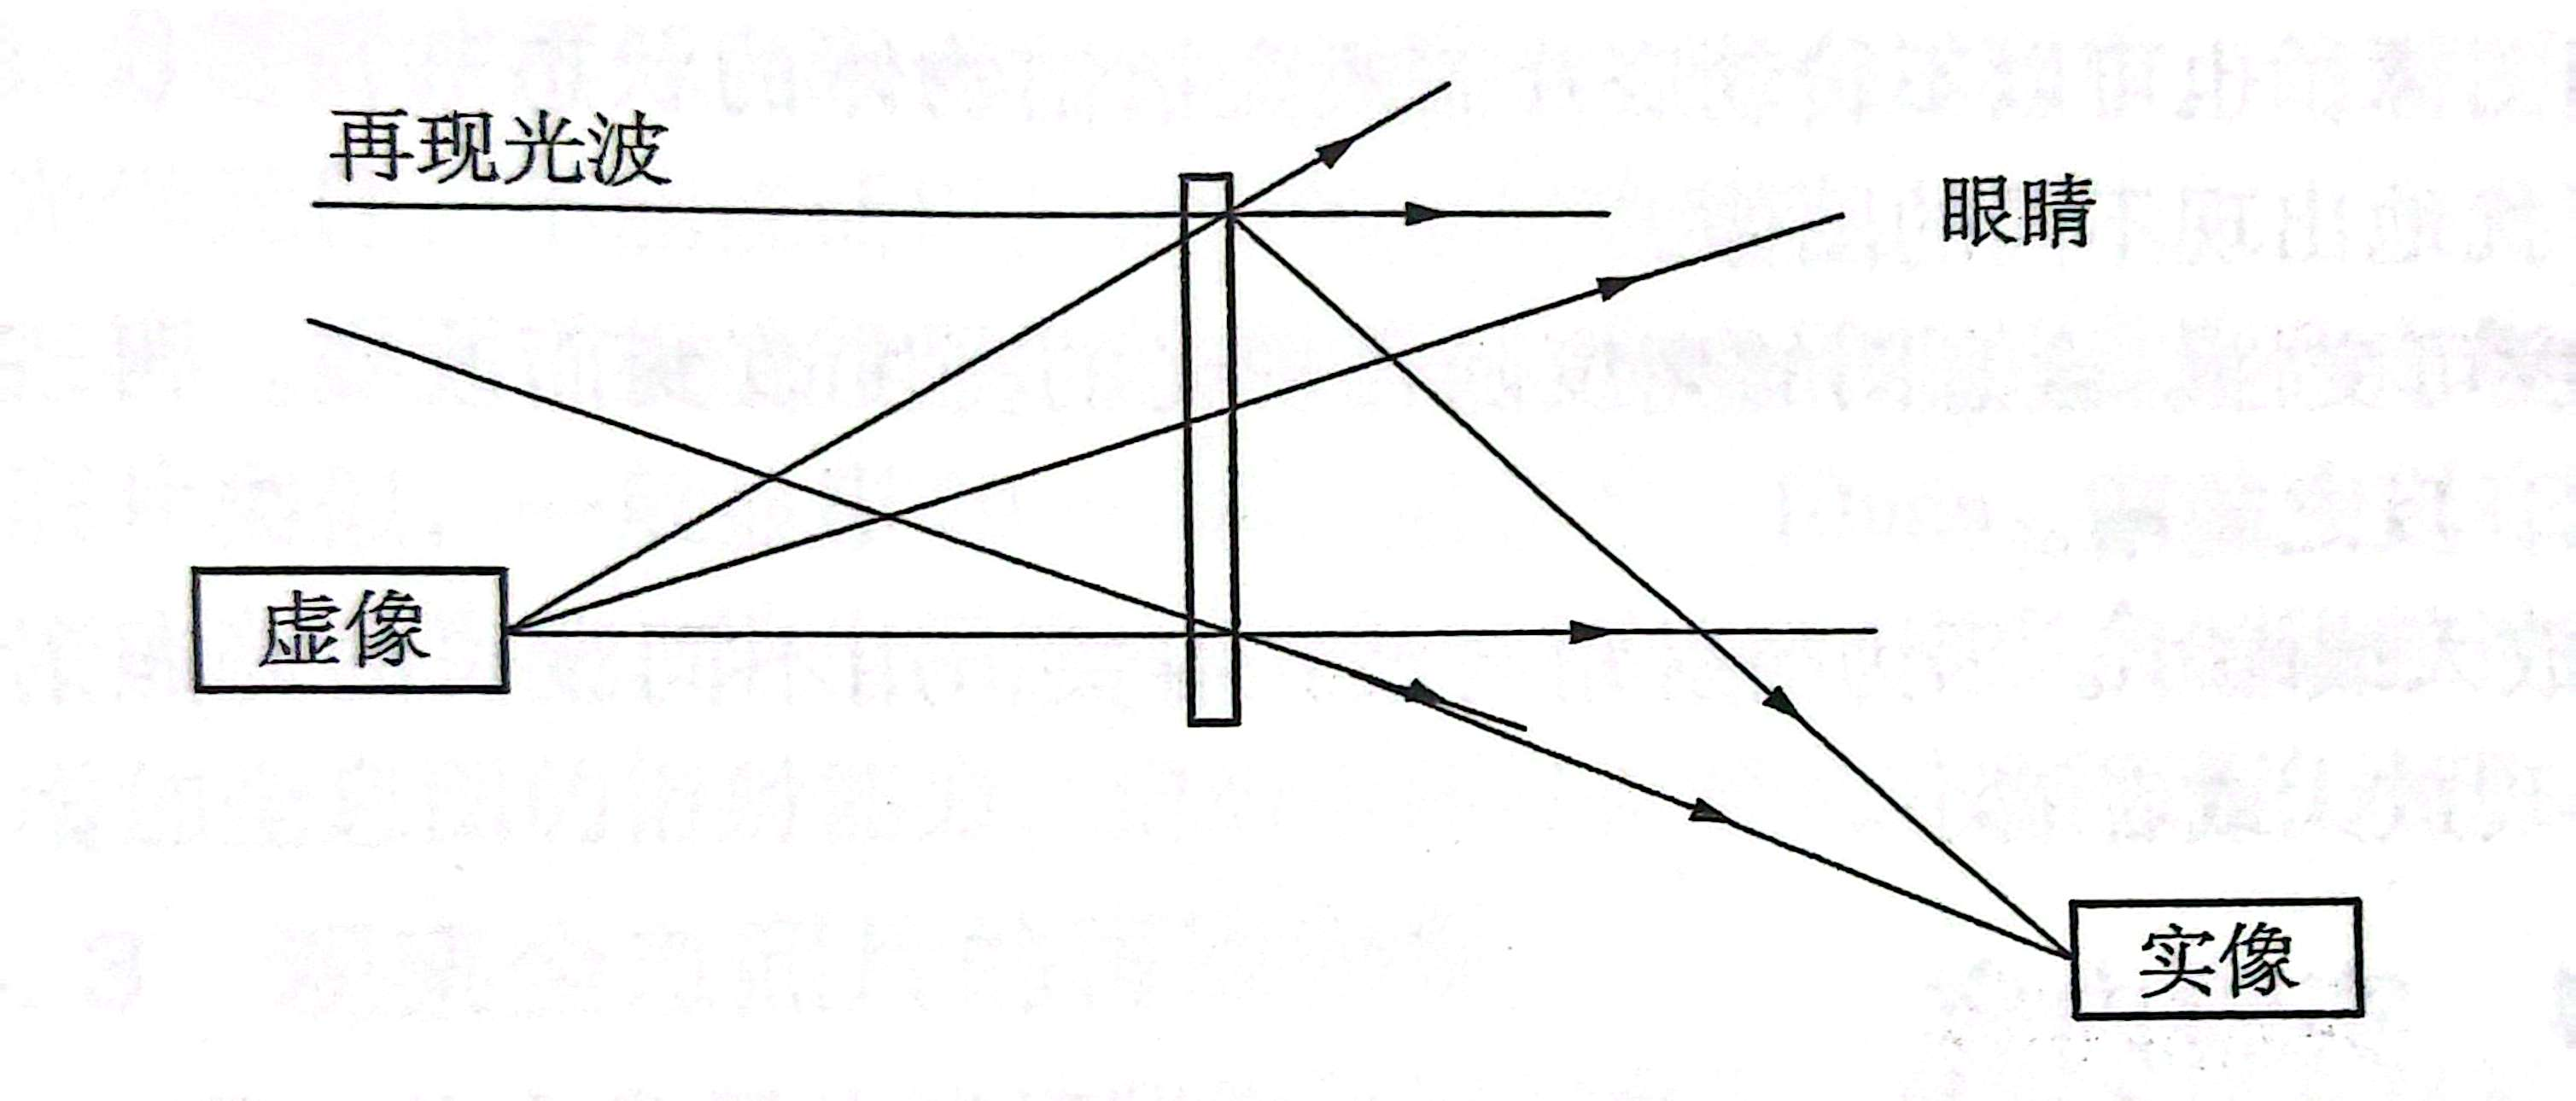
\includegraphics[width=0.6\textwidth]{assets/Figure_2.jpg}
    \caption{物像再现}
    \label{fig:holography_reconstruction}
\end{figure}

\textbf{5. 全息照片特点}

\begin{enumerate}
    \item \textbf{三维性}：因为全息图记录的是光波的全部信息，即振幅与相位同时记录在全息图上，图像具有显著的视差特性，可以看到逼真的三维图像。而普通图像只记录了振幅，得到的是二维平面图像。
    
    \item \textbf{可分割性}：全息照片被打碎后，它的任何一个碎片都能再现完整的被拍物体信息。因为全息照相过程中，物面和像面之间是点面对应的关系，形成的全息照片中每一个局部都包含了物像各点的信息。
    
    \item \textbf{信息容量大}：可以转动底片角度拍摄多次，再现时作同样转动不同角度可以出现不同图像，也可以不转动底片而改变被拍物体的状态进行多次曝光，再现时可以互不干扰地出现不同的图像。
    
    \item \textbf{亮度可变性}：全息图的亮度随再现光的亮度改变而改变。再现光越强，像的亮度越大，反之越暗。
    
    \item \textbf{可放大或缩小}：因为衍射角与波长有关，用不同波长的光照射全息图，再现像就会出现放大或缩小。
\end{enumerate}

\textbf{四、实验步骤}

\textbf{1. 调节全息照相光路系统}

根据全息照相实验的基本要求，在进行实验前要先了解、熟悉全息照相实验设备、仪器和光学元件支架的调整和使用方法。

\begin{enumerate}
    \item \textbf{调整实验台}：调整、检查光学实验台的水平度和稳定度。由于全息底片上所记录的干涉条纹很细，相当于波长量级，在照相过程中微小的干扰都会引起干涉条纹的模糊，不能形成全息图，因此要求整个光学系统的稳定性良好。对于全息实验台，进行检测、或在光学实验台上组合一个迈克尔逊干涉仪，干涉条纹在曝光时间内移动量小于四分之一到二分之一条纹间距，则基本满足实验条件。平台的水平度一般用气泡水准仪检查。

    \item \textbf{摆放光路}：按照图\ref{fig:holography_principle}摆放实验光路，并(1)使各元件基本等高共轴;在底片架上夹一块白屏，使参考光均匀照在白屏上，入射光均匀照亮被摄物体，且其漫反射光能照射到白屏上，调节两束光夹角在30°\textasciitilde45°之间;(3)使物光和参考光的光程大致相等，可分别挡住物光和参考光。调节其光强比，两光束有足够的重叠区;(4)所有光学元件必须通过摆放光与平台保持稳定.

    \item \textbf{检查实验光路}：开启激光电源并调节扩束镜和反射镜使物光和参考光充满感光屏。用测光仪器（代替感光屏）测量物光和参考光的相对强度（即分束比）。
\end{enumerate}

\textbf{2. 拍摄静态全息照片}

\begin{enumerate}
    \item 根据感光板的性质（即感光材料的分辨率和感光板的感光灵敏度）以及光源的强弱确定曝光时间，一般可选择10\textasciitilde15s。最好通过试拍确定最佳时间，然后再调整曝光计时器。

    \item 在输出镜前用一挡光板挡住光束，在底片夹上装夹全息干板。必须把涂有感光材料的一面（可以有手触摸干板边缘，相对不光滑的一面就是涂层）朝向物体以便接收物光。

    \item 静止数分钟后才可开启激光电源进行曝光。曝光过程中，绝对不能触碰防震台以及任何光学元件，不能说话以及在防震台周边走动。

    \item 曝光完毕，拆下干板进行显影定影处理。全息干板的显影和定影的处理过程与普通照相底片类似，一般显影20\textasciitilde30s，定影5\textasciitilde10min。实验中以在绿色灯光下观察到底片变为灰色为准，取出用流水冲洗3\textasciitilde5min，使多余的银粒冲去，用电吹风吹干。为增加全息图的衍射能力，定影后还可以对底片进行漂泊处理。
\end{enumerate}

\textbf{3. 观察全息照片的再现物像}

\begin{enumerate}
    \item \textbf{观察虚像}：将全息照片放回到原干板支架上，使涂有感光材料面朝向参考光（接收扩束束的激光束）。先遮住物光束，直接从全息照片背面观察（图\ref{fig:holography_reconstruction}），可以看到原物体位置上的虚像。

    \item \textbf{观察实像}：为了方便观察，通常直接利用扩束的激光照射全息照片的反面（非感光材料面），选取适当的角度观察，可得到比较清晰的实像。
\end{enumerate}

\textbf{五、数据处理与结果分析}

在光程计算方面，我们测量了两条主要光路的光程长度。物象光程通过16.5cm + 16cm + 28.5cm的叠加计算得到总光程为61cm。另一条光路的光程计算为32cm + 21cm + 11.5cm，总光程为64.5cm。需要特别说明的是，第一条光路中的16.5cm路径包含分光镜进行分光，因此在计算中需要考虑分光镜对光程的影响。两条光路的光程差为3.5cm，这个差值在氦氖激光器的相干长度范围内，确保了良好的干涉效果。

\begin{figure}[H]
    \centering
    \begin{minipage}{0.45\textwidth}
        \centering
        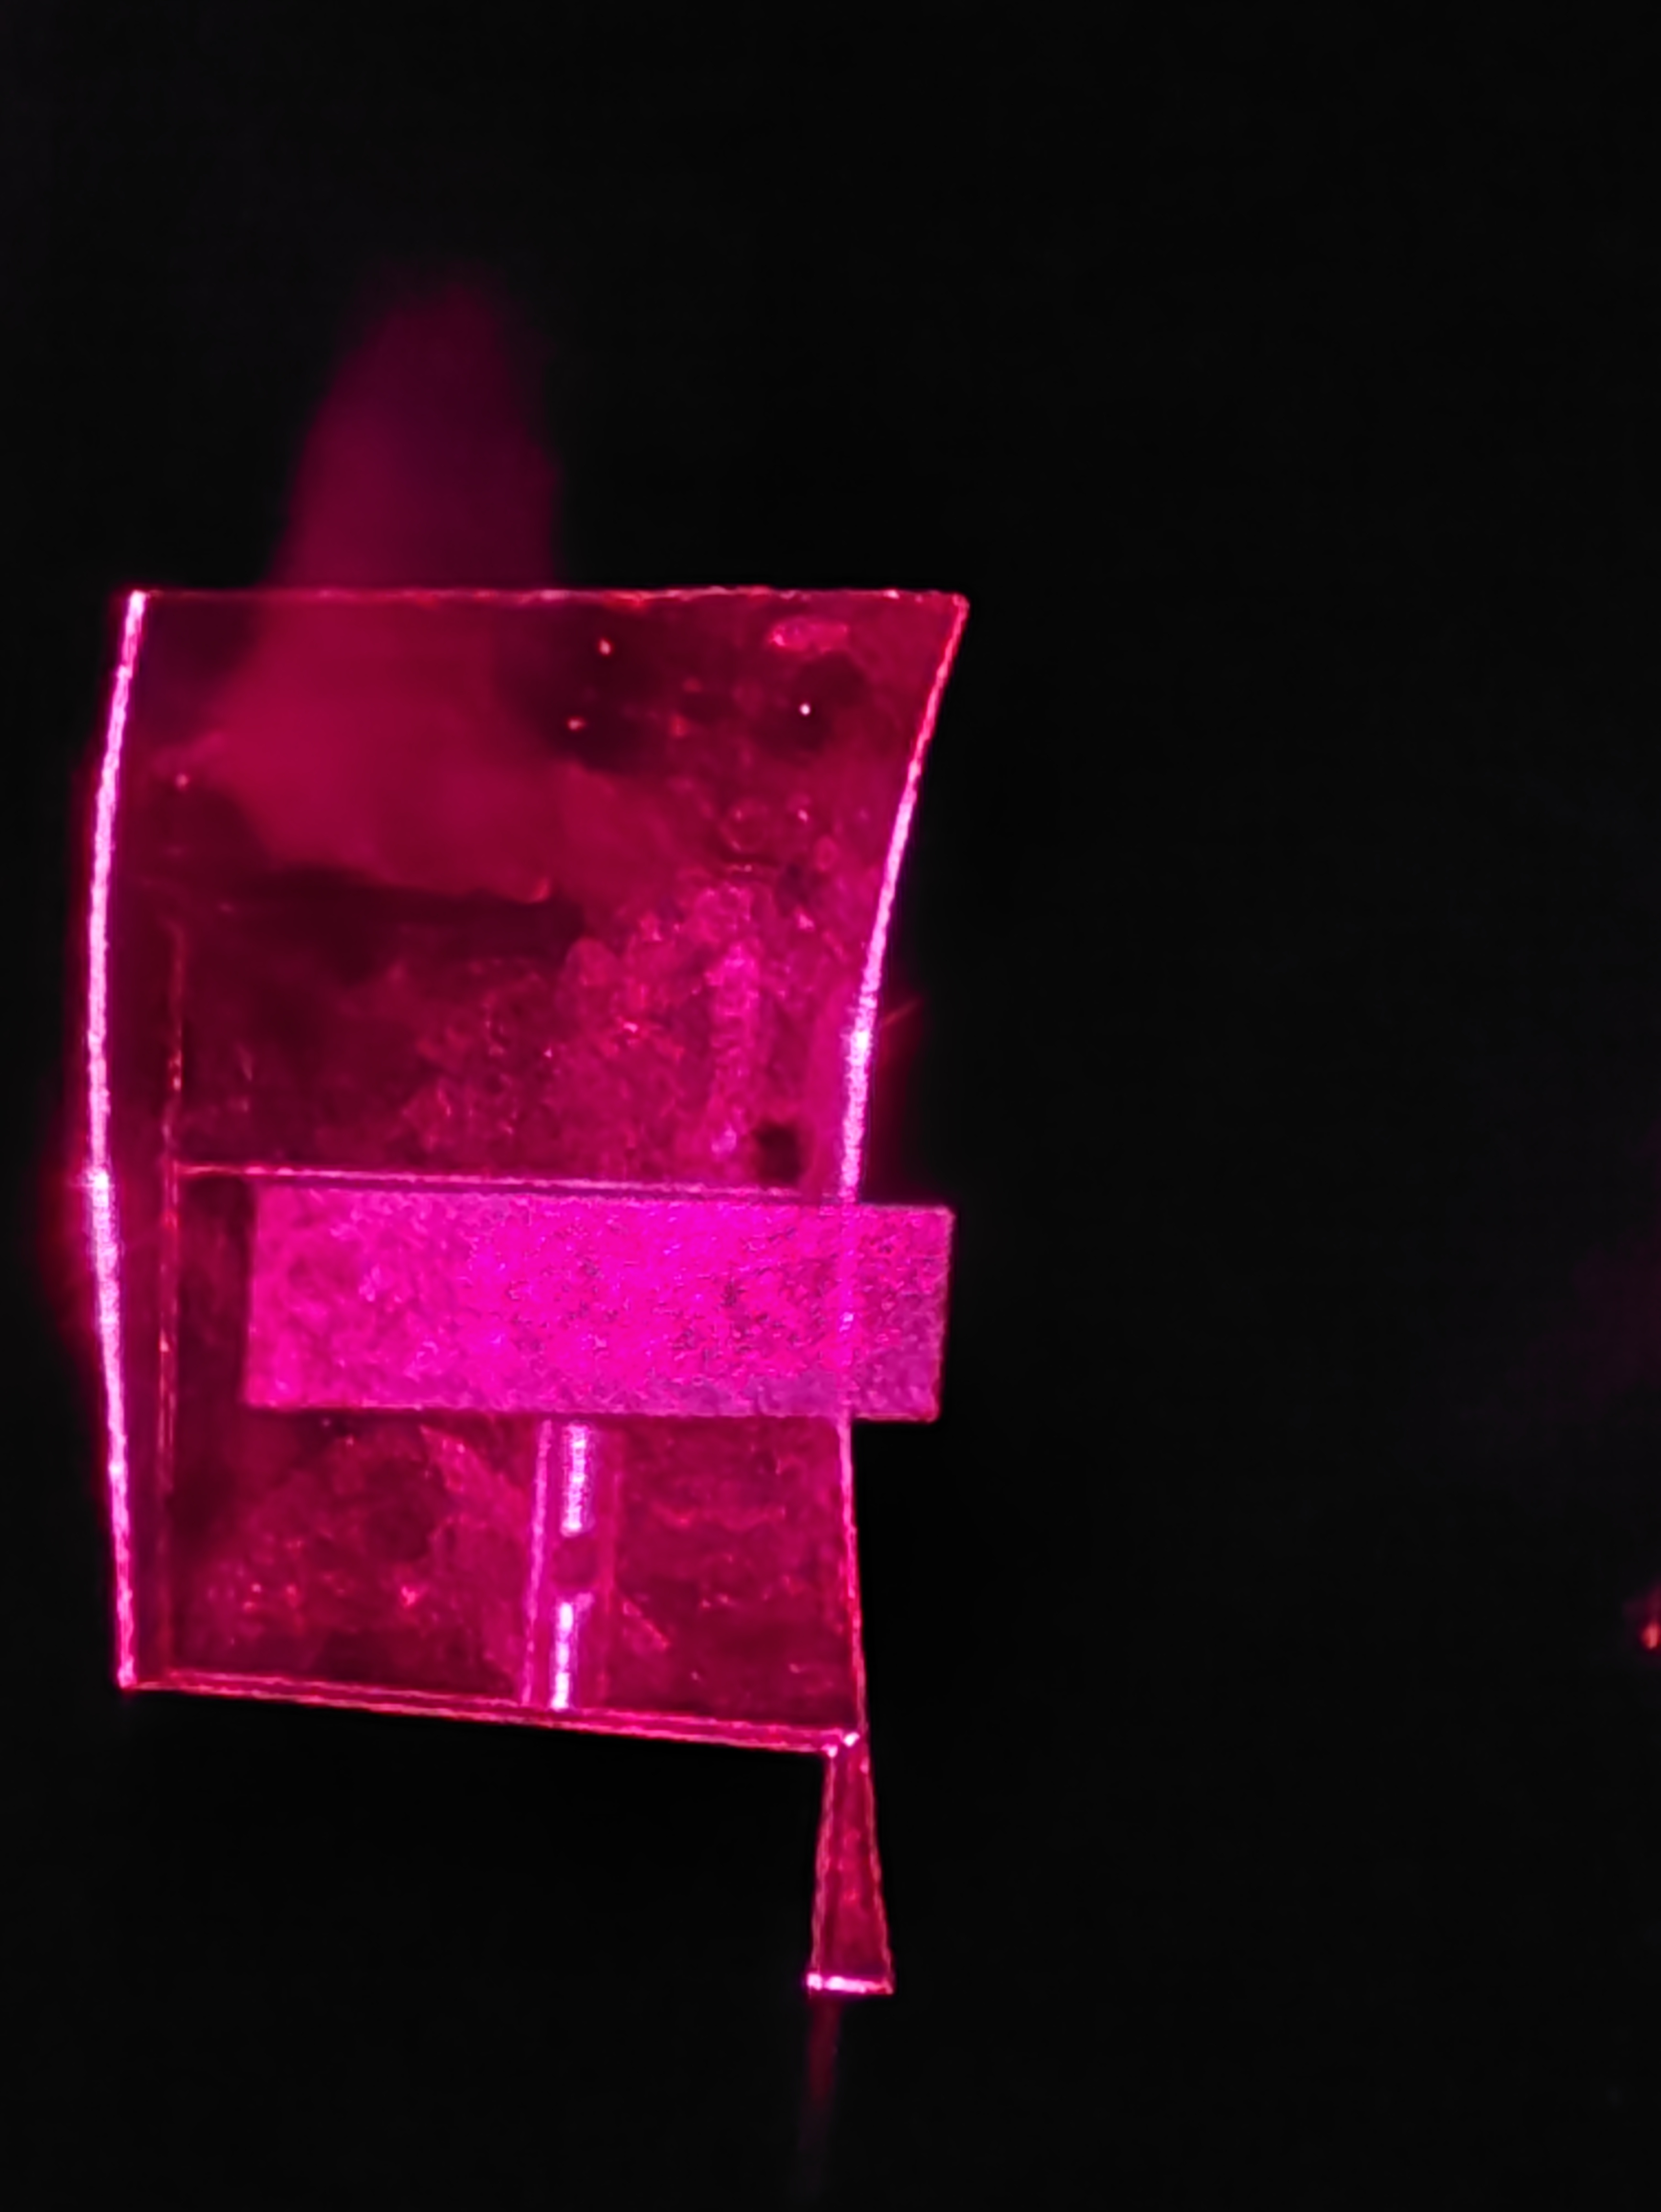
\includegraphics[width=\textwidth]{assets/IMG_20250909_103733.jpg}
        \caption{全息照片虚像观察}
    \end{minipage}
    \hfill
    \begin{minipage}{0.45\textwidth}
        \centering
        \includegraphics[width=\textwidth]{assets/IMG_20250909_100433.jpg}
        \caption{全息照片实像观察}
    \end{minipage}
\end{figure}

观察结果显示全息照相实验取得了良好的效果。在虚像观察过程中，图像非常清晰，立体感很强，视差效果十分明显。当改变观察角度时，能够清楚地看到物体的不同侧面，充分体现了全息照相的三维特性。实像观察相对来说亮度较暗一些，但仍然具有较好的清晰度和明显的视差效果。由于使用单色激光再现，观察到的像呈现红色单色特征。

全息照片的质量分析表明实验达到了预期目标。制作出的全息照片具有显著的立体效果，观察时能明显感受到物体的三维立体感，这是全息技术区别于普通照相技术的重要特征。图像清晰度良好，特别是在虚像观察时图像非常清晰，实像虽然相对较暗但仍能清楚辨认物体的细节特征。再现像的位置非常准确，虚像出现在原物体所在位置，实像在全息板另一侧的预期位置出现，这验证了全息再现的基本原理。

通过实验验证了全息照片的主要特性。三维性体现在具有明显的立体感和视差效果上，当观察者移动位置时能看到物体的不同角度。可分割性通过用小片全息板观察得到验证，即使是很小的一块全息片仍能看到完整的物像，这说明全息图的每一部分都包含了整个物体的信息。亮度可变性在调节再现光强度时得到体现，像的亮度随着再现光强度的变化而相应改变。

\textbf{六、结论和讨论}

本次全息照相实验成功制作了质量良好的激光全息照片，充分验证了全息照相的基本原理。通过实际操作，我们观察到了全息照片的主要特点，包括三维立体效果、真实的空间位置关系以及完整的信息记录能力。实验过程中掌握了全息照相的关键技术，包括光路的调节和稳定性控制、曝光参数的选择和精确控制、全息底片的专业处理技术以及全息像的正确观察方法。

\textbf{七、思考题解答}

关于光程差的思考题，许多实验教材强调物光波和参考光波的光程差要很小甚至要接近相等，如果使光程差比较大如20cm或40cm，并不一定得不到全息图。光程差大小主要影响的是对激光相干长度的要求，而激光的相干长度可以用公式$L_c = \frac{\lambda^2}{\Delta\lambda}$来计算，其中$\Delta\lambda$是激光的线宽。对于质量良好的氦氖激光器，相干长度通常可以达到几十厘米甚至更长，因此20cm或40cm的光程差在激光的相干长度范围内是完全可以接受的。虽然理论上光程差较大仍能形成全息图，但在实际操作中光程差过大会增加对激光稳定性的要求，使系统更容易受到温度变化和机械振动的影响，同时可能导致干涉条纹对比度有所下降。在实验中可以通过逐步增加光程差来验证这一理论，观察全息图质量随光程差变化的规律。

对于在没有激光进行再现的条件下如何检查干板上是否记录了信息的问题，有多种可行的方法。白光观察法是最简单直观的方法，用白炽灯或自然光照射全息板，调整观察角度寻找彩虹色的衍射光，如果能看到彩色光谱分布就说明全息板上记录了信息。密度测量法通过使用光学密度计测量全息板的透光密度，与未曝光的空白板进行对比，密度的变化表明有干涉条纹信息被记录下来。显微镜观察法可以直接观察全息板表面的微细结构，寻找肉眼无法直接看到的干涉条纹图案，条纹的存在直接证明了信息的成功记录。还可以尝试使用其他具有一定相干性的单色光源如LED或汞灯等进行照明观察，虽然效果不如激光理想，但在某些条件下仍可能观察到再现像。这些检验方法为在缺乏激光设备的情况下判断全息记录的成功与否提供了有效的手段。

\textbf{八、实验心得}

通过本次全息照相实验，我深刻理解了全息技术的科学原理和实际应用价值。实验过程中最大的挑战是保持系统的稳定性，任何微小的振动都可能影响最终结果。这让我认识到精密光学实验对环境条件的严格要求。

全息技术作为一项重要的光学技术，在现代科技中有着广泛的应用前景。从基础的三维显示到先进的信息存储，全息技术都展现出独特的优势。实验让我不仅掌握了全息照相的基本技能，更重要的是培养了严谨的科学态度和实验操作能力。

\end{document}
